\documentclass[11pt]{article}
%\documentclass{book}
\usepackage[utf8]{inputenc}
\usepackage[T1]{fontenc}
\usepackage[french]{babel}
\usepackage[top=1.8cm, bottom=1.8cm, left=1.8cm, right=1.8cm]{geometry}
\usepackage[linktocpage,colorlinks=false]{hyperref}
\usepackage{graphicx}
\usepackage{epsfig}
\usepackage{amssymb}
\usepackage{amsmath}
\usepackage{array}
\usepackage{subfig}
\usepackage{multicol}
\usepackage{caption}
\usepackage{listings}
\usepackage{algorithm}
\usepackage{algorithmic}
\hypersetup{
    colorlinks=true,
    breaklinks=true,
    urlcolor=red,
}
\parskip=5pt

\title{\huge{\textbf Compte Rendu}}
\author{AYOUB Pierre, BASKEVITCH Claire, BESSAC Tristan, \\
CAUMES Clément, DELAUNAY Damien, DOUDOUH Yassin}
\date{Mercredi 18 Avril 2018}

\begin{document}

\maketitle
\vspace{20em}
\begin{center}
\includegraphics{pictures/Application.png}\end{center}
\newpage

\tableofcontents

\newpage

\section{Introduction}

La stéganographie est le but recherché lors de l'implémentation de StegX. 
ELle consiste à dissimuler des données dans des fichiers de type image, 
audio et vidéo. 
Après avoir étudié en détail les algorithmes de stéganographie (dans le 
cahier des charges), et analysé comment mettre en relation les différents 
modules correspondant aux différentes fonctionnalités, il est maintenant 
temps d'implémenter le logiciel.
L'application StegX proposera à ses utilisateurs de manipuler une interface 
graphique ou en ligne de commandes afin de cacher des données dans d'autres 
données (pour des formats pris en charge par StegX). De plus, StegX permettra 
d'extraire des données d'un fichier que l'on considère déjà comme cachant 
des données. Le logiciel proposera plusieurs algorithmes de stéganographie
tels que EOF, LSB et Metadata. 

En plus de l'implémentation, il sera utile de présenter le fonctionnement 
de l'architecture de l'application avec les explications techniques. 
Une description des points délicats seront mis en valeur ainsi qu'un 
bilan technique sur l'application et humain sur l'équipe de conception. 

\section{Architecture du produit}

\hspace{0.5cm}
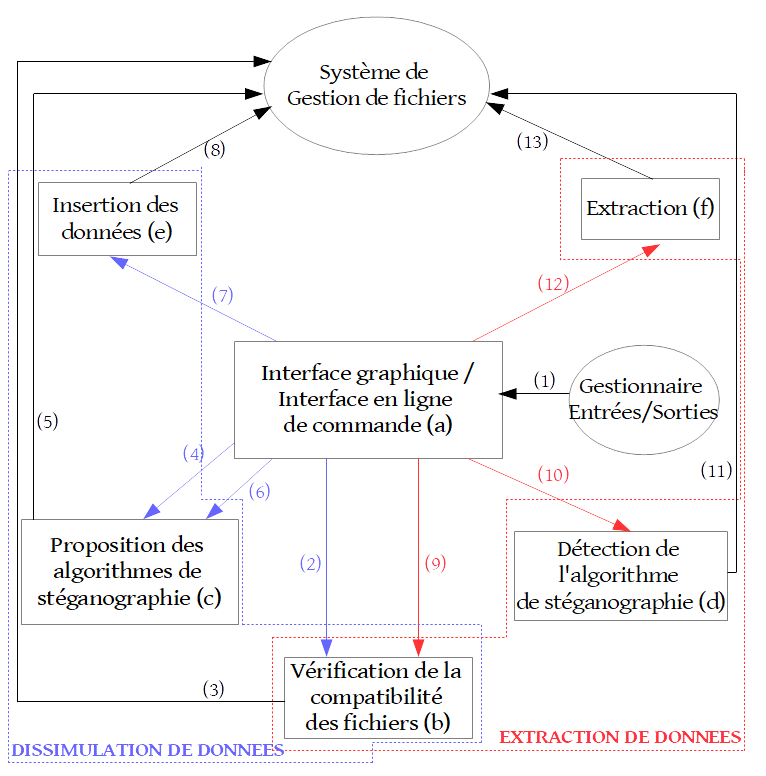
\includegraphics[scale=0.55]{pictures/organigramme.png}
\newpage

L'étude des différentes propriétés de la stéganographie et la stéganalyse 
nous a mené vers cet organigramme. 
Il permet de visualiser les étapes successives de la stéganographie 
(insertion des données), ainsi que celle de la stéganalyse (extraction 
des données). 

Pour la dissimulation de données, il va d'abord y avoir la vérification 
de la compatibilité du fichier hôte, pour savoir si le format est bien 
pris en charge par l'application. 
Il y a ensuite, le module \textit{Proposition des algorithmes de stéganographie}
qui va être utilisé. Un premier appel vers ce module permettra de proposer 
un ou plusieurs algorithmes en fonction du fichier hôte et du fichier à cacher. 
Puis, le deuxième appel permettra à l'utilisateur de choisir l'algorithme 
parmi ceux proposés précedemment. 
La dernière étape consiste en la réelle insertion des données, où les 
données à cacher seront dissimulées dans une copie du fichier hôte. 

Pour l'extraction de données, le module \textit{Vérification de la compatibilité 
des fichiers} permettra, comme pour l'insertion, de vérifier si le format 
du fichier à analyser est bien pris en charge. 
Il y aura ensuite une détection de l'algorithme de stéganographie permettant de 
trouver la méthode utilisée par l'émetteur pour cacher les données. 
Enfin, l'extraction permettra de récupérer les données cachées dans le 
fichier à analyser. 

Tous ces modules et sous-modules seront coordonnées grâce aux interfaces 
graphique et en ligne de commande, proposées par StegX. 




\section{Explications techniques}

\section{Description du fonctionnement}

Pour montrer le fonctionnement de l'application, nous allons proposer un 
exemple pour dissimulation et un autre pour l'extraction, correspondant 
à une communication entre Alice et Bob, surveillée par Oscar. 
Les données sont issues d'une réelle utilisation de StegX. 

\subsection{Fonctionnement de l'insertion des données dans un exemple}

Alice choisit de dissimuler le message dans une image qu'elle veut envoyer 
à Bob à l'aide de l'interface graphique. 
Tout d'abord, elle choisit les entrées de la dissimulation : le fichier 
à cacher, le fichier hôte ainsi que le chemin du fichier à créer et un mot 
de passe pour augmenter la sécurité de la dissimulation. 
Dans cet exemple, le fichier à cacher est /home/user/Bureau/message.txt 
de taille 2.2 kB ; le fichier hôte est /home/user/Images/photo.bmp 
de taille 21.1 MB ; le chemin du fichier à créer est 
/home/user/Documents/piece\_jointe.bmp ; le mot de passe est "alicebob" 
(communiqué à Bob sur un canal sûr). 

L'interface va appeler le module \textit{Vérification de la compatibilité 
des fichiers}. Le type du fichier hôte sera analysé grâce à la lecture 
de l'entête du fichier : il s'agit d'un fichier BMP non compressé dont les 
pixels sont codés sur 24 bits (8 bits par composantes couleurs). 
Le sous-module \textit{Proposition des algorithmes de stéganographie} va 
remplir la structure spécifique 
\textit{infos.host.file\_info.bmp}, notamment avec le 
\textit{header\_size} égal à $122$ octets, le \textit{data\_size} égal à 
$21085440$ octets, le champ \textit{pixel\_length} égal à $24$ et le champ 
\textit{pixel\_number} égal à $2584 \times 2720 = 7028480$. De cette structure
est déduit les algorithmes proposés (EOF, LSB et Metadata). 
Dans cet exemple, Alice choisit l'algorithme EOF. 

La prochaine étape est celle de l'insertion. Pour la stéganographie EOF, 
StegX va écrire dans /home/user/Documents/piece\_jointe.bmp le fichier hôte. 
Ensuite, la signature StegX est écrite dans lequel on a l'identificateur 
de l'algorithme (1 octet), la taille du fichier caché noté en Big Endian 
(sur 4 octets), la taille du nom du fichier caché (1 octet) et le nom du 
fichier caché XOR avec le mot de passe "alicebob" choisi au début (255 octets 
maximum). 
Enfin, les données cachées sont également écrites avec le XOR du mot de passe. 

Alice pourra donc envoyer le fichier piece\_jointe.bmp qui aura une taille 
de 21088071 octets soit 21.1 MB sur un canal non sécurisé. 

Oscar, qui espionne les communications entre Bob et Alice, n'aura aucun 
soupçons en voyant piece\_jointe.bmp qui semble être une image comme une 
autre. 

\subsection{Fonctionnement de l'extraction des données dans un exemple}

Bob reçoit sur le canal non sûr le fichier piece\_jointe.bmp et sait que 
ce fichier contient des données cachées. Pour les extraire, Bob choisit 
d'utiliser StegX avec l'interface en ligne de commande. 

Il tape dans son terminal \textit{stegx -e -o piece\_jointe.bmp -r 
/home/user/Bureau/ -p alicebob} qui signifie que Bob veut extraire les 
données cachées du fichier piece\_jointe.bmp, que le résultat de ces 
données extraites doivent être écrites dans son Bureau et que Bob veut 
extraire les données cachées à l'aide du mot de passe "alicebob"

Tout d'abord, le module \textit{Vérification de la compatibilité des 
fichiers} va analyser le type de piece\_jointe.bmp. Il s'agira bien du 
format BMP non compressé. 

Ensuite, le module \textit{Détection de l'algorithme de stéganographie}
permettra de remplir la structure spécifique de \textit{infos.host.file\_info.bmp}
et déduira les mêmes champs que Alice lors de l'insertion. En effet, 
il va y avoir une lecture approfondie du fichier. Ensuite, la signature 
StegX, qui a été écrite lors de l'insertion, sera lu pour ne déduire 
le nom du fichier caché, l'algorithme et la taille du fichier caché. 

Enfin, le module \textit{Extraction}, appelé par l'interface, va réaliser 
l'extraction. Ici, les données cachées ont été XOR avec "alicebob" choisi 
par Alice lors de l'insertion et nécessaire pour l'extraction effectuée 
par Bob. 
Les données cachées extraites seront écrites dans le fichier
/user/home/Bureau/message.txt. Bob pourra ainsi lire le message de Alice 
contenu dans le fichier message.txt. 

\section{Description des points délicats de la programmation}

\section{Comparaison estimation - implémentation}

\small
\hspace{-1cm}
\begin{tabular}{|c|c|c|c|}
  \hline
  \textbf{Module de l'application} & \textbf{Coût en nombre de lignes} & \textbf{Coût en temps} & \textbf{Personnel(s) en charge} \\
  \hline
    Interface en ligne & Estimation : 200 lignes & Estimation : 30 heures & BASKEVITCH Claire \& \\ 
    de commande & Implémentation : X lignes & Implémentation : X heures & BESSAC Tristan \\
  \hline
  Interface & Estimation : 400 lignes & Estimation : 30 heures & AYOUB Pierre \& \\
  graphique & Implémentation : X lignes & Implémentation : X heures & DELAUNAY Damien \\
  \hline
  Vérification de la & Estimation : 300 lignes & Estimation : 30 heures& CAUMES Clément \& \\
   compatibilité des fichiers & Implémentation : X lignes & Implémentation : X heures & DOUDOUH Yassin \\
  \hline
    Proposition des algos & Estimation : 100 lignes & Estimation : 15 heures & CAUMES Clément \& \\
   de stéganographie & Implémentation : X lignes & Implémentation : X heures & DOUDOUH Yassin \\
  \hline
    Détection de l'algo & Estimation : 100 lignes & Estimation : 15 heures & AYOUB Pierre \& \\
   de stéganographie & Implémentation : X lignes & Implémentation : X heures & DELAUNAY Damien \\
  \hline
  Dissimulation \& Extraction & Estimation : 250 lignes & Estimation : 40 heures & CAUMES Clément \& \\
   fichiers images & Implémentation : X lignes & Implémentation : X heures & DOUDOUH Yassin \\
  \hline
  Dissimulation \& Extraction & Estimation : 250 lignes & Estimation : 40 heures & AYOUB Pierre \& \\
   fichiers audios & Implémentation : X lignes & Implémentation : X heures & DELAUNAY Damien \\
     \hline
  Dissimulation \& Extraction & Estimation : 250 lignes & Estimation : 40 heures & BASKEVITCH Claire \& \\
   fichiers vidéos & Implémentation : X lignes & Implémentation : X heures & BESSAC Tristan \\
  \hline
\end{tabular}
\normalsize

\section{Bilan du produit}

Le produit StegX répond bien aux objectifs : faire de la stéganographie 
et de la stéganalyse sur des fichiers de type image, audio et vidéo en 
utilisant plusieurs algorithmes (LSB, EOF, Metadata). 
Par ailleurs, StegX propose bien 2 interfaces : une en ligne de commande 
et une autre graphique. 
Avoir choisi le langage C a été le meilleur choix car ce langage nous a 
permis de manipuler facilement les données binaires des fichiers en entrée. 

En plus de répondre aux objectifs, l'équipe de conception s'est efforcée 
à répondre aux nombreux besoins du client, qui doit rester la personne la 
satisfaite du produit. 

\section{Conclusion sur l'organisation interne au sein du projet}

Durant le semestre 6 de la dernière année de licence informatique à Versailles, 
l'équipe StegX s'est réuni pour créer une application en rapport à la 
cryptographie. 
De ce fait, tous les membres de l'équipe de conception se sont efforcés à
travailler de façon professionnelle et ordonnée. En effet, ils leur tenaient 
à coeur de mettre en application toute la méthodologie informatique acquise 
durant la Licence. 
Par ailleurs, en raison de la grande charge de travail, il a fallu, dès le 
début du projet, de diviser la conception selon les trois différents types 
dont StegX doit se charger (image, audio et vidéo). 
Cette division de charge de travail impliquait que chacun devait réaliser 
une partie de la conception. 

Enfin, nous n'avions pas de chef de projet. Cette décision nous a été très 
favorable du fait que chacun a eu la maturité de comprendre les enjeux de 
ce grand projet. En effet, ces enjeux étaient grands et c'est pour cela 
que le projet IN608 est la matière la plus travaillée du semestre. 

\end{document}
